% !TEX root = ../main.tex
% --+ 20.04 FMT EFFICIENCY STUDY +----------------------------------------------
\begin{frame}{FMT Efficiency Study}
    \label{20.04::fmt_efficiency_study}
    \begin{itemize}
        \item
            Then, to see how these efficiency effects affects the different DIS variables, we need to understand their behavior in

            \vspace{6pt}
            \begin{itemize}
                \item
                    vertex z position (\ef{$v_z$}),

                \item
                    polar angle (\ef{$\theta$}),

                \item
                    azimuthal angle (\ef{$\varphi$}), and

                \item
                    momentum (\ef{$p$}).
            \end{itemize}

        \vspace{12pt}
        \item
            Based on the geometry cut, we expect a strong dependence on \ef{$v_z$} and \ef{$\theta$}, and at most a weak one on \ef{$\varphi$} and \ef{$p$}.
    \end{itemize}

    \vspace{12pt}
    \ef{*}All plots presented in this appendix are from \ef{run 12016}.

    \backref{11.44::reconstruction_effect}
\end{frame}

\begin{frame}{FMT Efficiency Study: $v_z$}
    \begin{center}
        \vspace{-6pt}
        \begin{figure}[t]
            \centering{
                \fbox{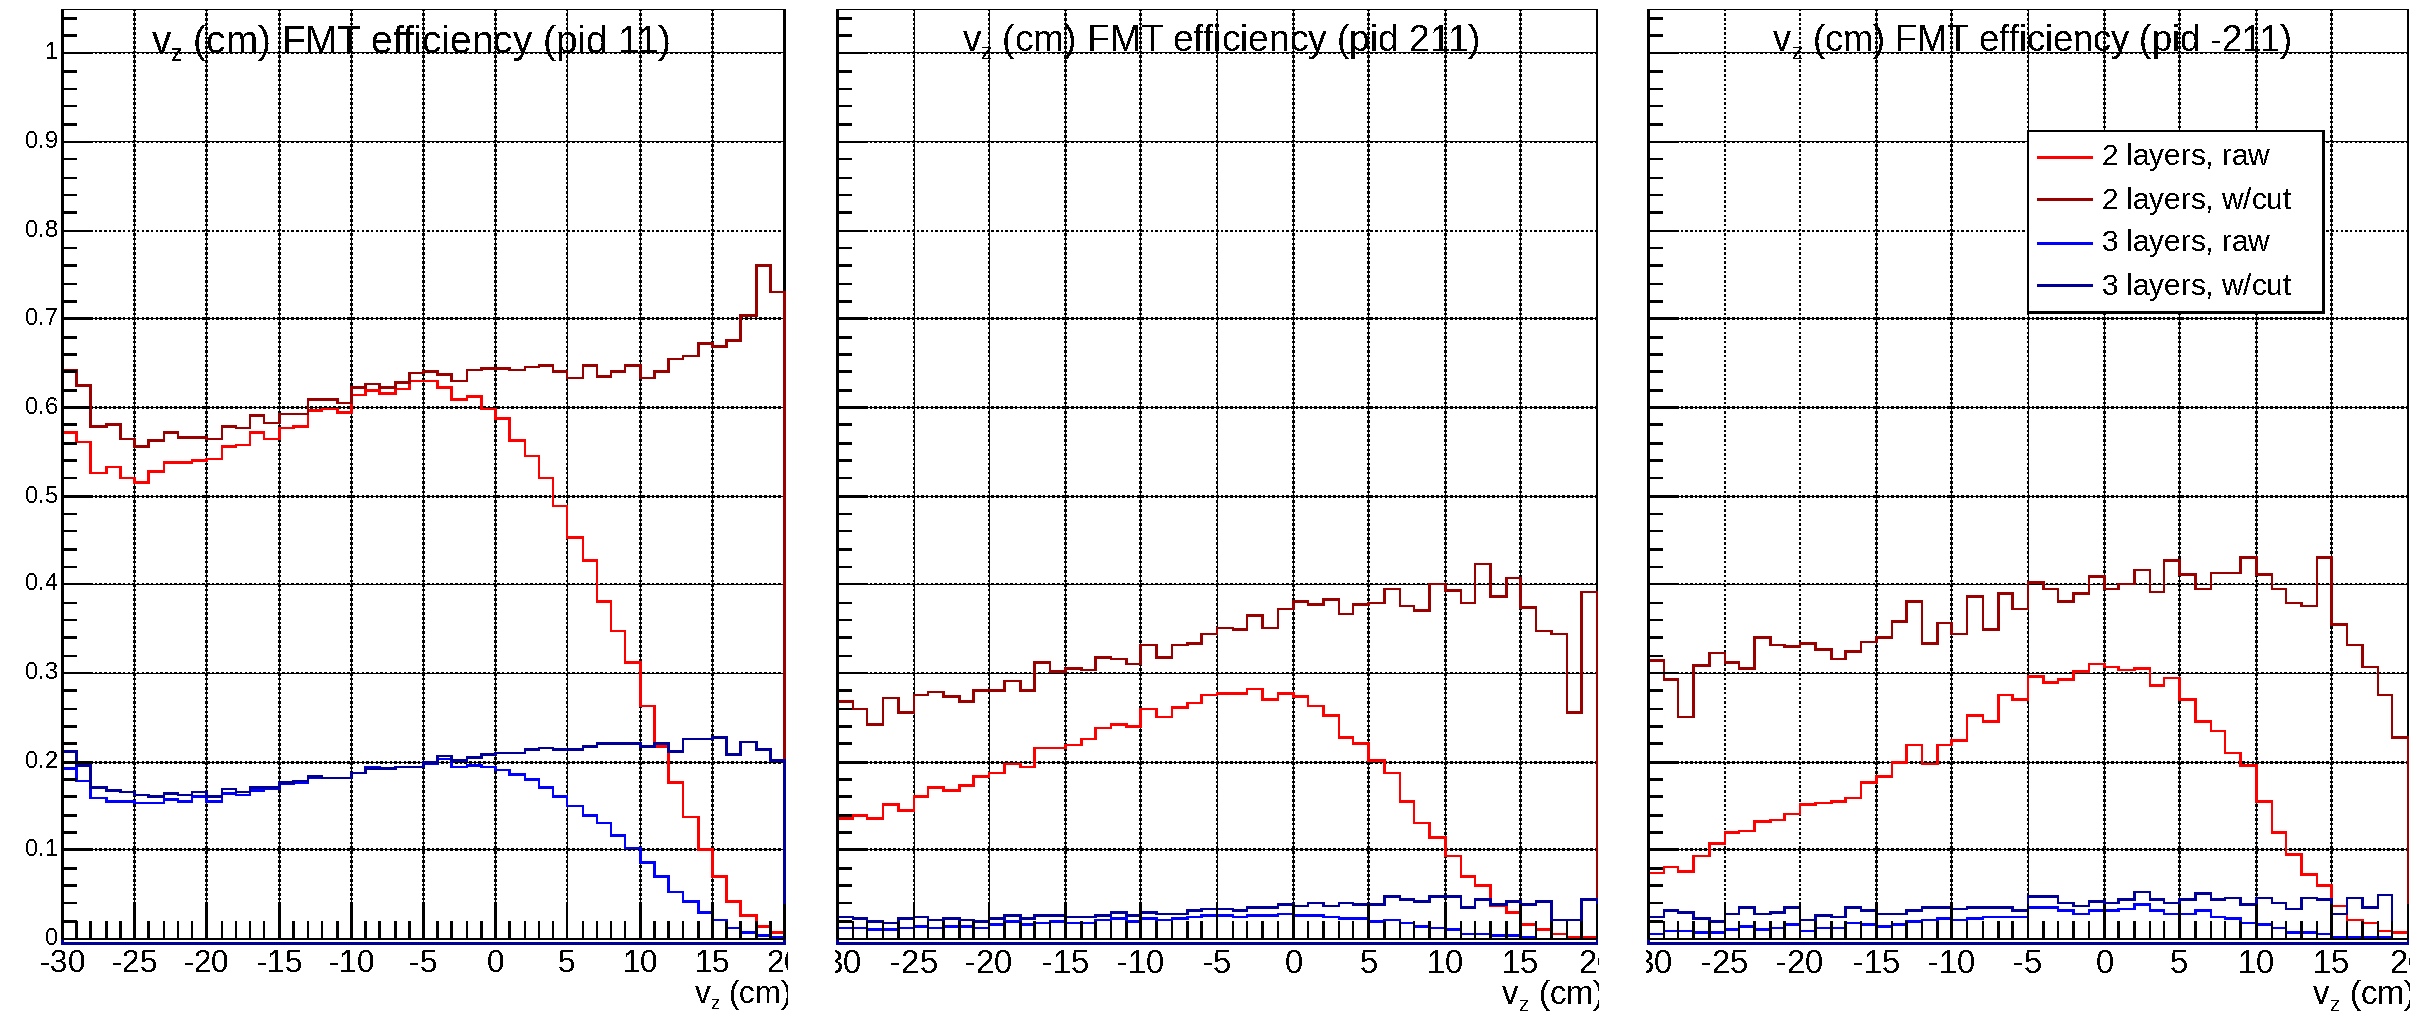
\includegraphics[width=0.98\textwidth]{04eff_vz.pdf}}
            }
        \end{figure}
        \textit{Efficiency over \ef{$v_z$} for $e^-$, $\pi^+$, and $\pi^-$}
    \end{center}

    \backref{11.44::reconstruction_effect}
\end{frame}

\begin{frame}{FMT Efficiency Study: $\theta$}
    \begin{center}
        \vspace{-6pt}
        \begin{figure}[t]
            \centering{
                \fbox{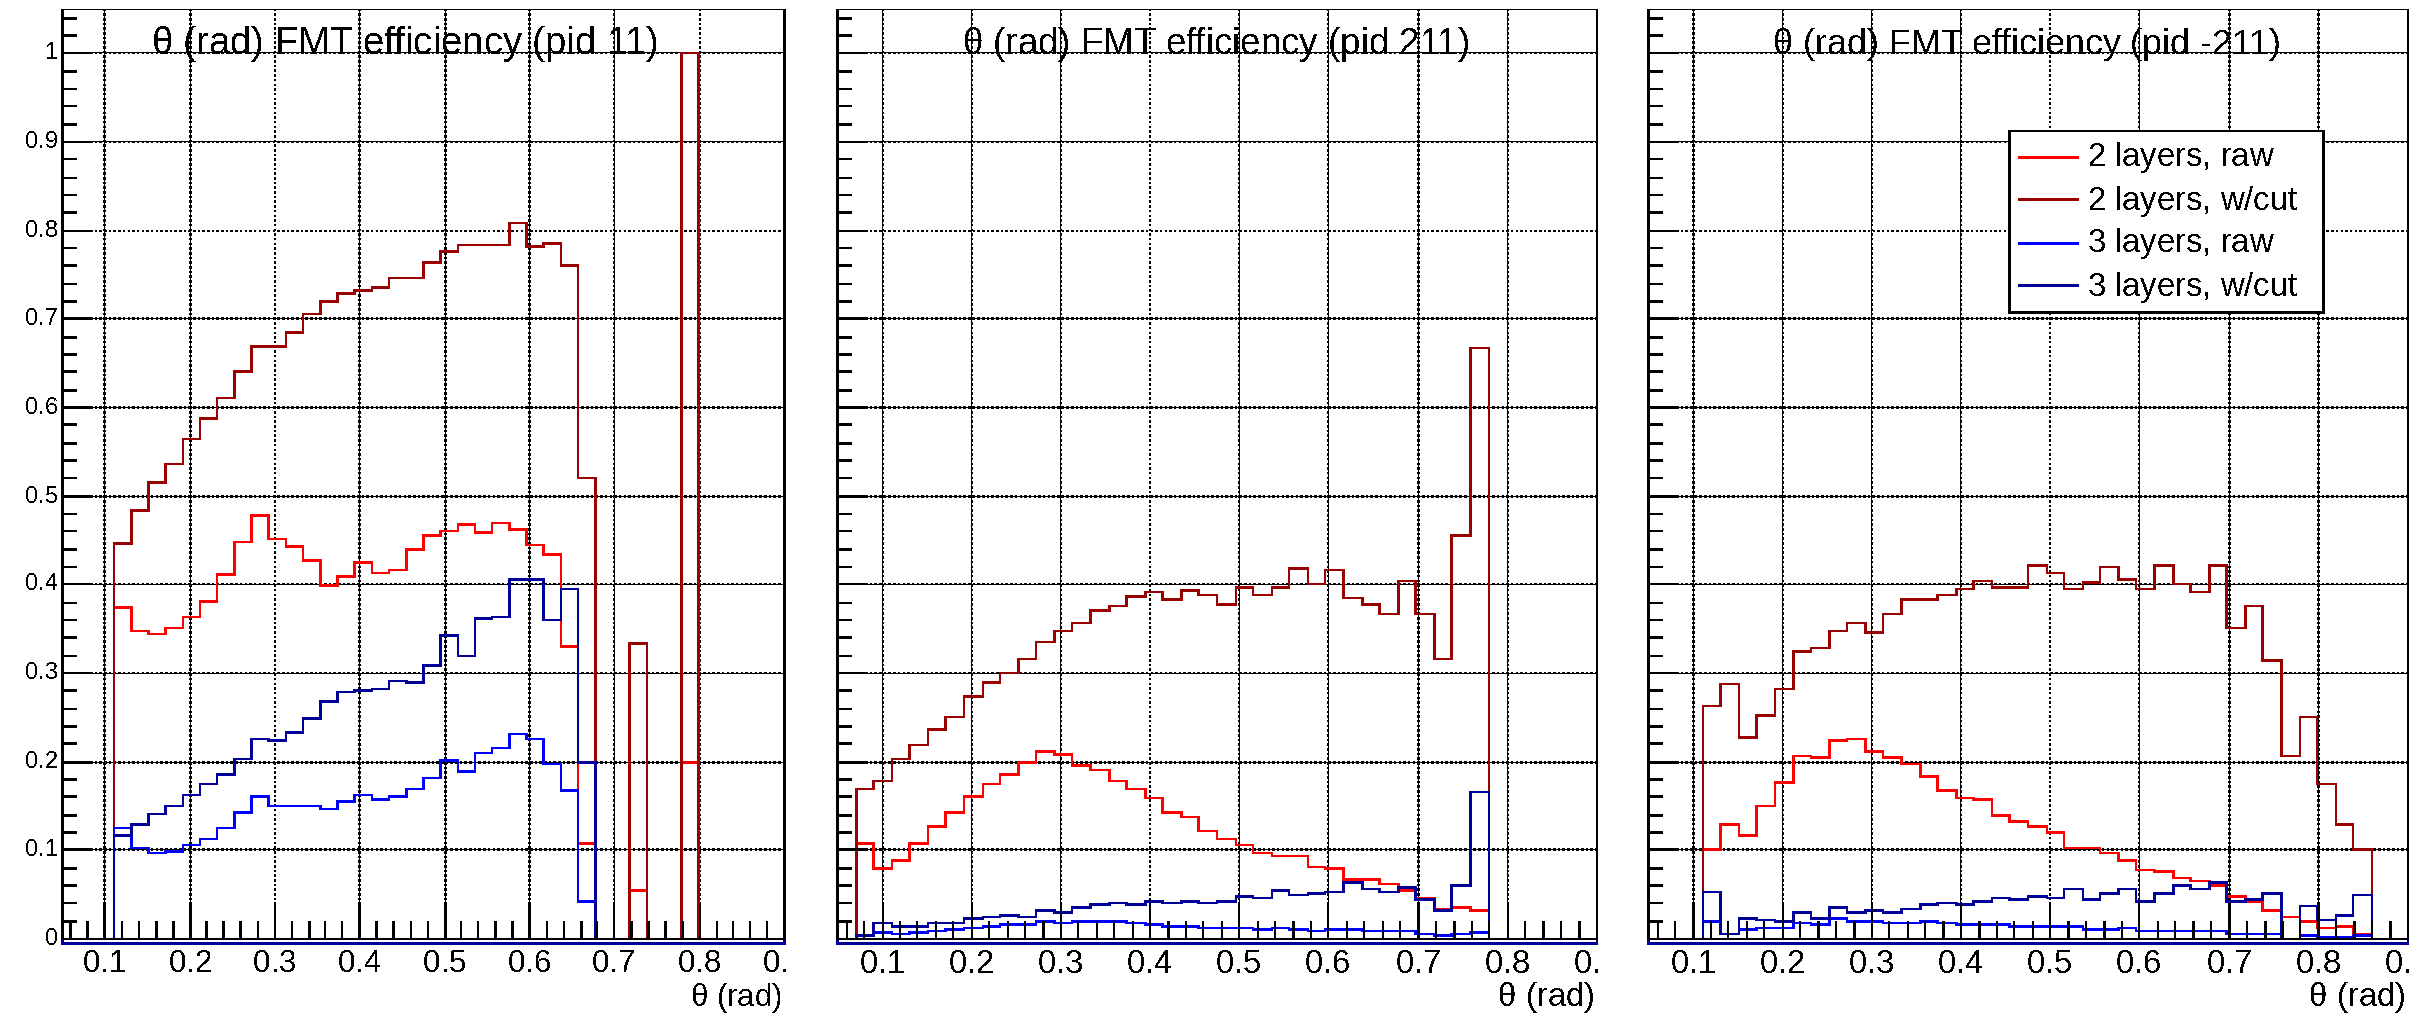
\includegraphics[width=0.98\textwidth]{04eff_theta.pdf}}
            }
        \end{figure}
        \textit{Efficiency over \ef{$\theta$} for $e^-$, $\pi^+$, and $\pi^-$}
    \end{center}

    \backref{11.44::reconstruction_effect}
\end{frame}

\begin{frame}{FMT Efficiency Study: $p$}
    \begin{center}
        \vspace{-6pt}
        \begin{figure}[t]
            \centering{
                \fbox{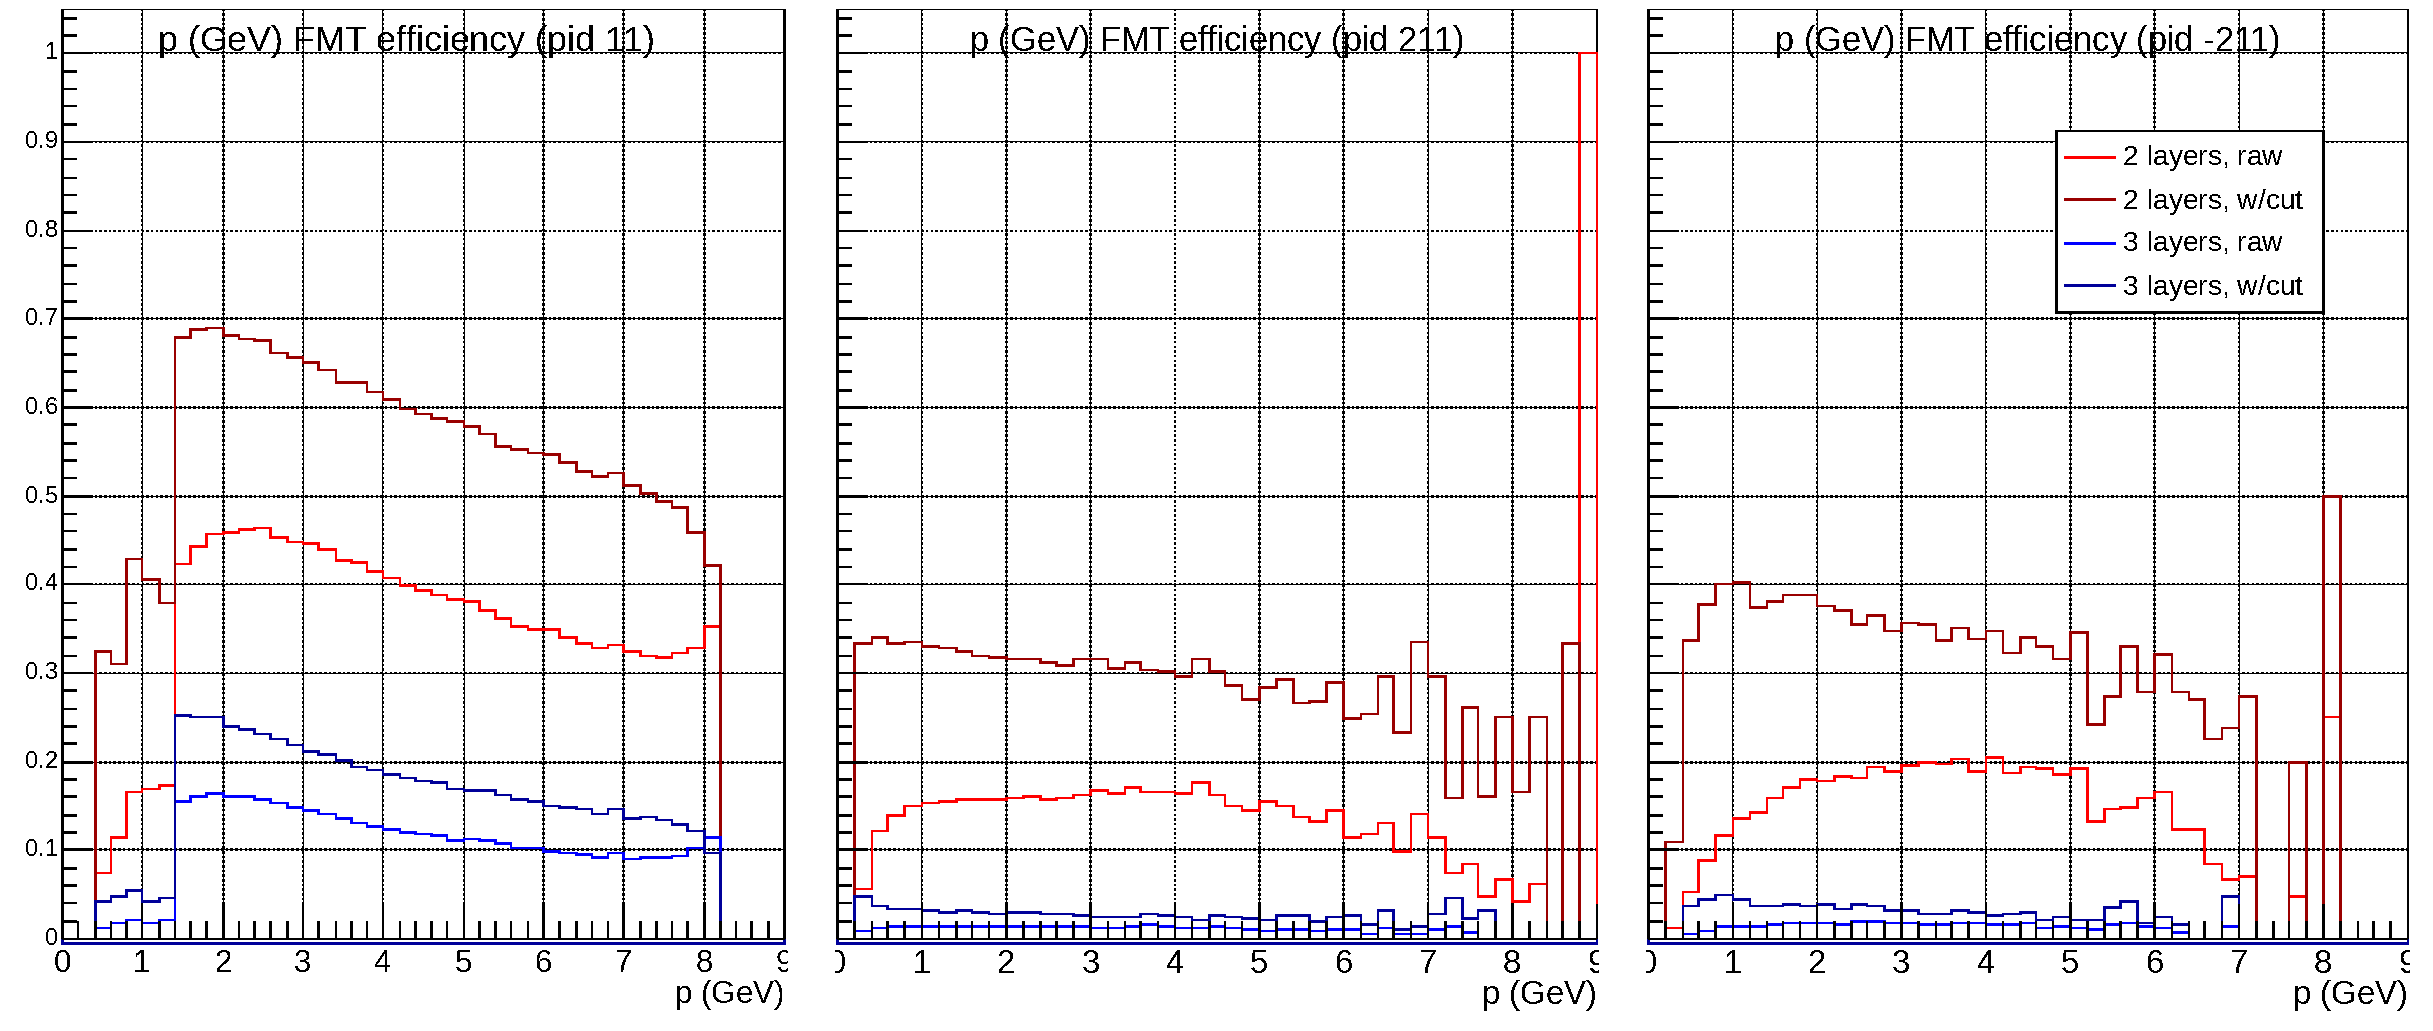
\includegraphics[width=0.98\textwidth]{04eff_p.pdf}}
            }
        \end{figure}
        \textit{Efficiency over \ef{$p$} for $e^-$, $\pi^+$, and $\pi^-$}
    \end{center}

    \backref{11.44::reconstruction_effect}
\end{frame}

\begin{frame}{FMT Efficiency Study: $\varphi$}
    \begin{center}
        \vspace{-6pt}
        \begin{figure}[t]
            \centering{
                \fbox{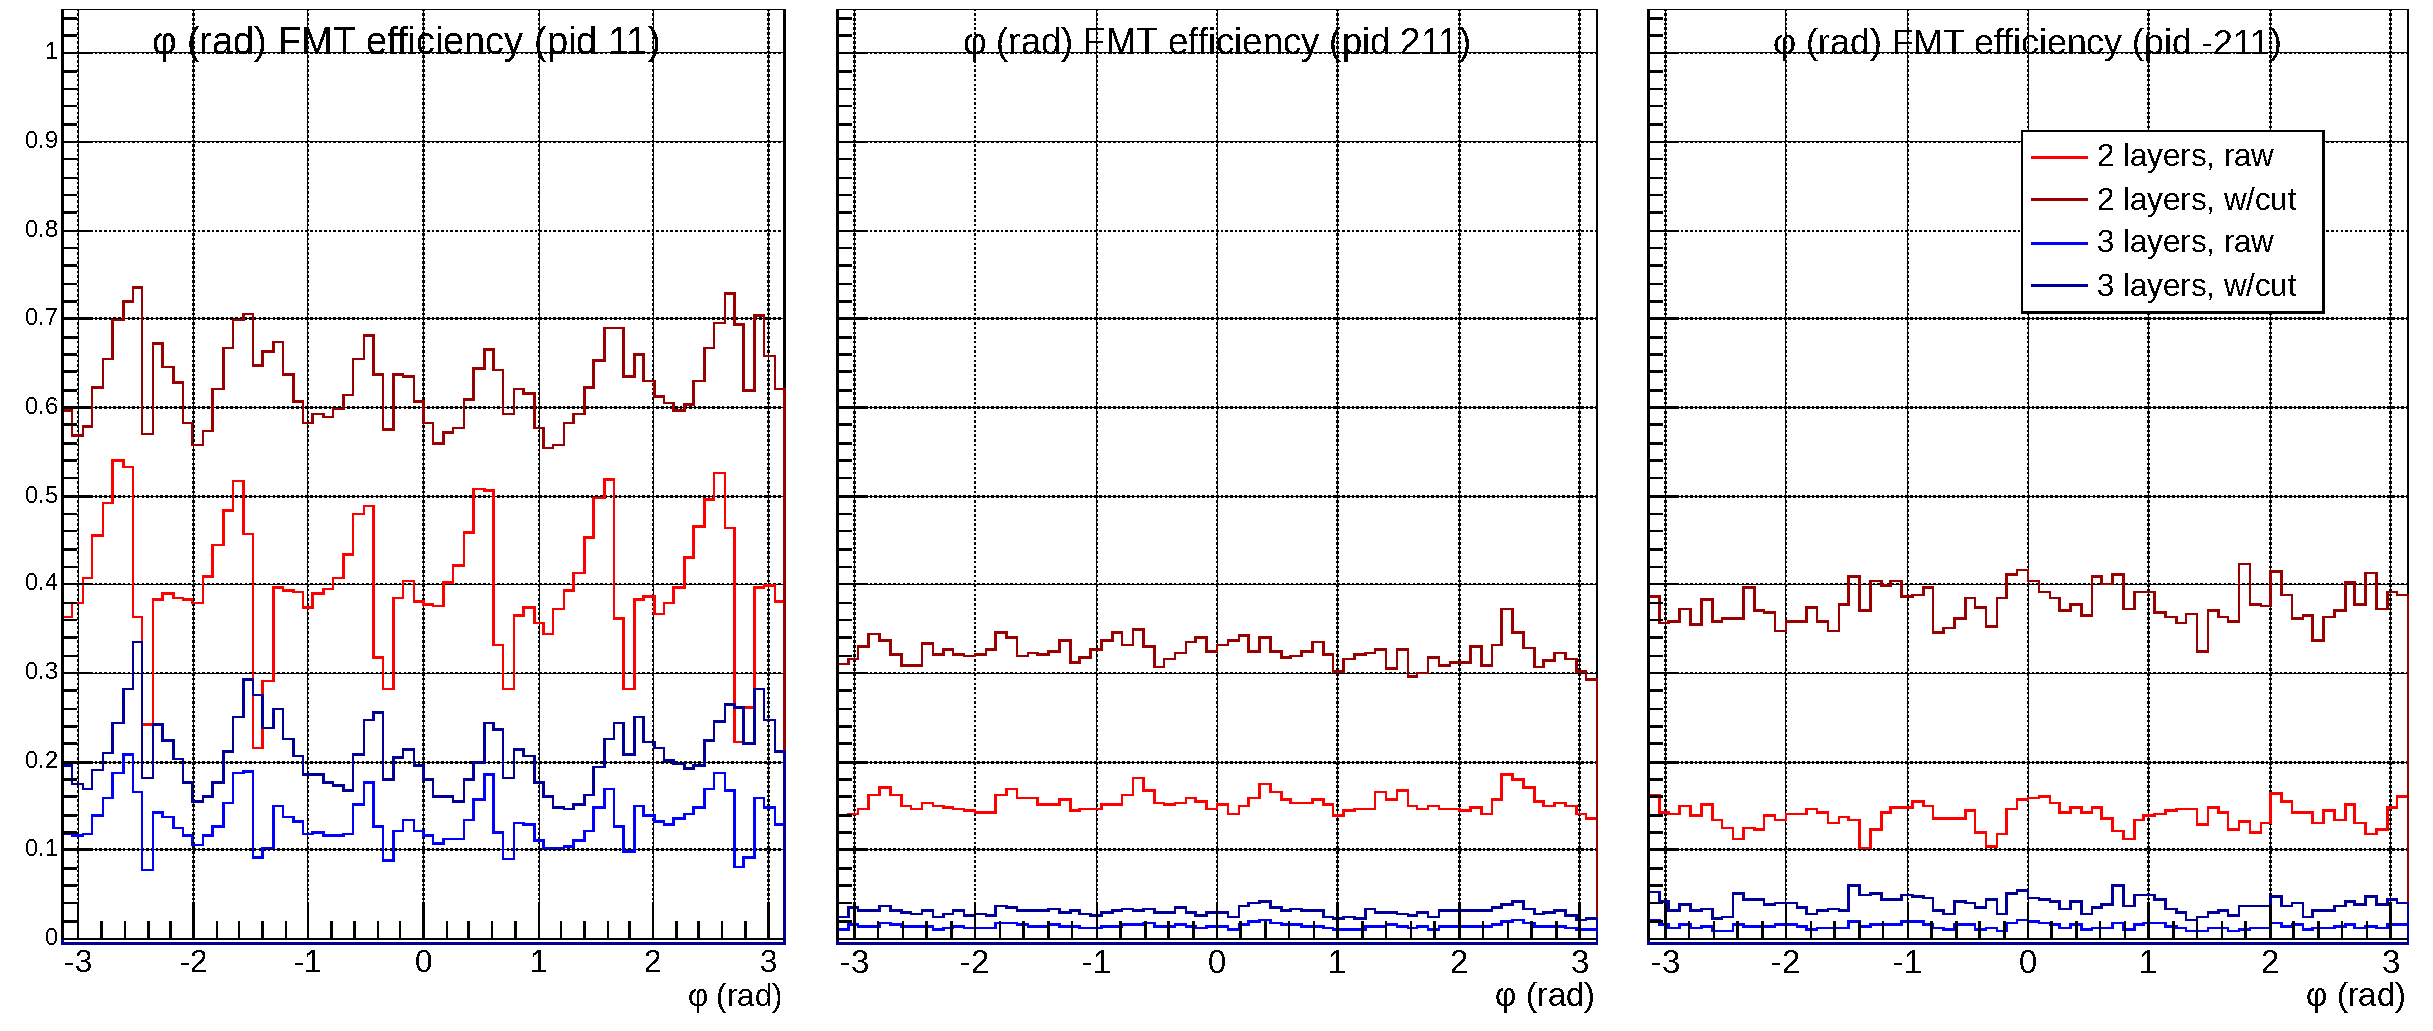
\includegraphics[width=0.98\textwidth]{04eff_phi.pdf}}
            }
        \end{figure}
        \textit{Efficiency over \ef{$\varphi$} for $e^-$, $\pi^+$, and $\pi^-$}
    \end{center}

    \backref{11.44::reconstruction_effect}
\end{frame}

\begin{frame}{FMT Efficiency Study: $\varphi$}
    \label{20.04::fmt_efficiency_study_end}

    The loss of the sharp dips in $e^-$ $\varphi$ efficiency can be explained by the loss of DC tracks upon applying the cut.

    \begin{center}
        \begin{figure}[t]
            \centering{
                \fbox{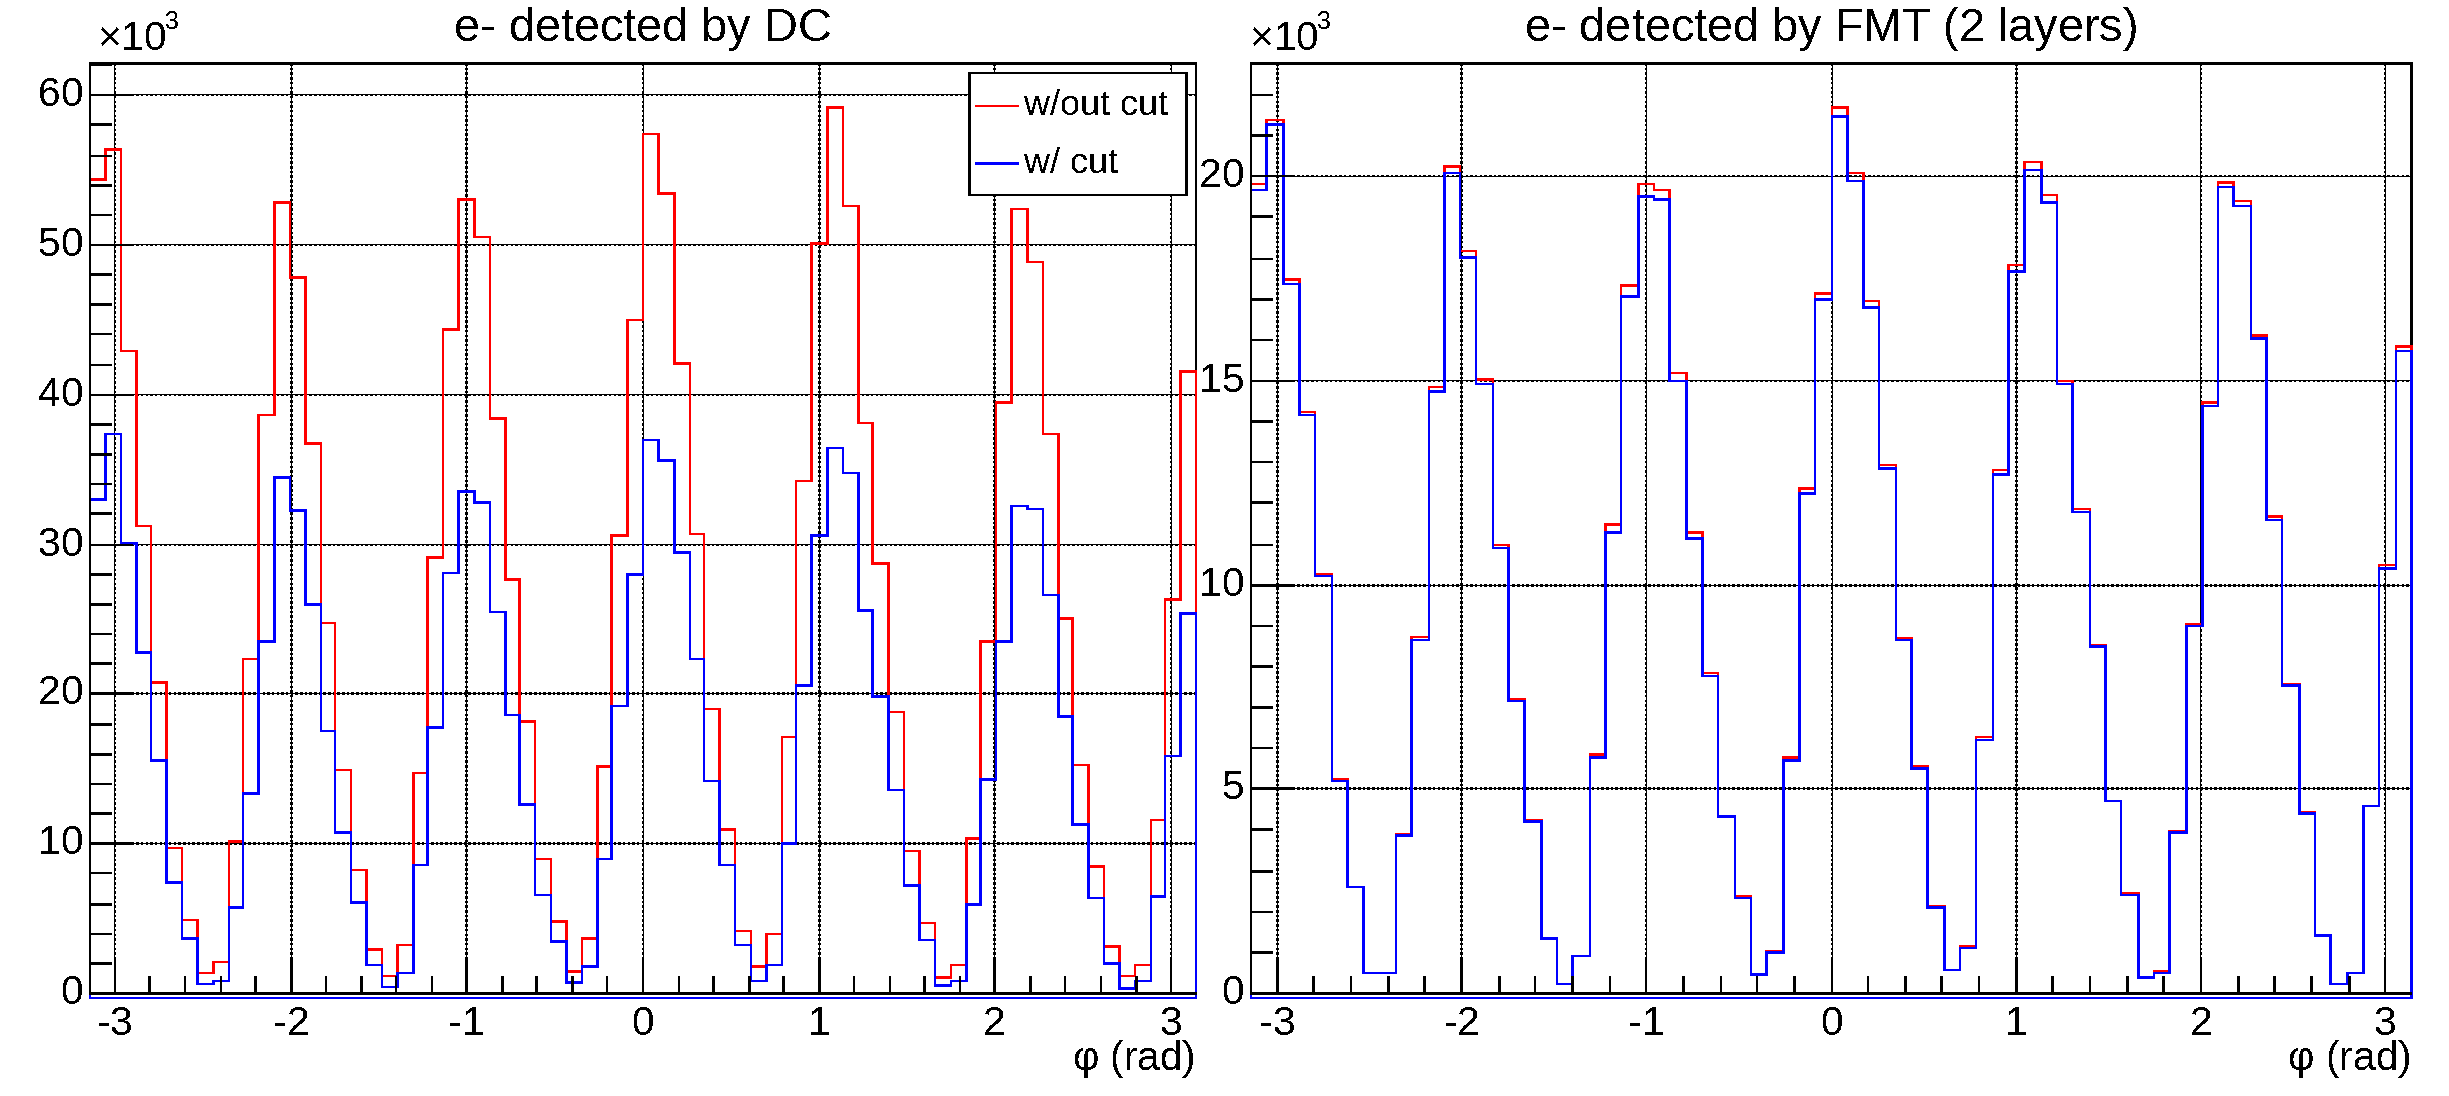
\includegraphics[width=0.98\textwidth]{04gcut_phi.pdf}}
            }
        \end{figure}
    \end{center}

    \backref{11.44::reconstruction_effect}
\end{frame}
